%Klynge, procesanalyse

\section{Procesanalyse}
\begin{frame}{Procesanalyse}{}
	\begin{itemize}
		\item Planlægning
        \begin{itemize}
            \item Trello
            \item Tidsplan
        \end{itemize}
		\item Uddelegering af arbejde
        \begin{itemize}
            \item Først til mølle
            \item Efter interesse
            \item Leo var helt alene, det er sgu da også synd!
        \end{itemize}
	\end{itemize}
  
  \begin{figure}
    \centering
    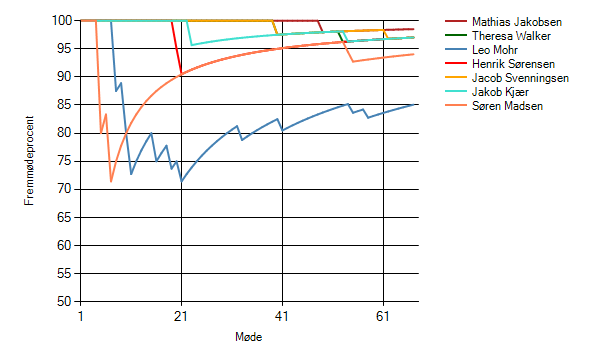
\includegraphics[width=.6\textwidth]{figures/graph.png}
  \end{figure}
  
  \note{
    Trello til referater og dagsordener.
    Grove tidsplaner
    
    Ledte til uddelegering af arbejde
      Antal personer
      
      Først til mølle
      Efter interesse
      Enligt medlem
  }
\end{frame}
%Arbejde i vores egen gruppe

%   Vi planlagde vores arbejde lidt af gangen. I store træk. 
%   F.eks. procesanalysen for sig selv.

%   Vi lavede en meget grov tidsplan i starten, men efterfølgende ikke rigtigt. 
%   Vi planlagde højst et par uger frem.

%   Trello blev brugt lidt svingende. 
%   Vi havde tænkt os, at bruge det til referater, dagsordener og planlægning v.h.a. små kort for hver opgave, der kunne farves, når opgaverne var færdige.
%   Endte med primært at være en platform til referater og dagsordner, fra vores vejledermøder og ugentlige gruppemøder. 
%   Vi kunne sagtens have gjort mere ud af tidsplanlægningen med Trello, ved f.eks. at udnævne en person til at holde styr på Trello evt. i en uge af gangen.
%   Om vi havde fået så meget produktivitet ud af det, er svært at sige.

%   Vores største problem var at vi blev distraheret af diverse ting og hurtigt faldt i snak. Om tidsplanlægningen kunne have hjulpet på dette er tvivlsomt.

%Uddelegering af arbejdet

%   Foregik lidt på først til mølle princippet, men dermed jo også efter hvad der interesserede folk, eller hvad de syntes de kunne overskue, da de forskellige opgaver havde variende sværhedsgrad
%   Leo var alene, det var nok noget vi skulle have taget op halvvejs igennem og snakket lidt mere om.

\section{Klyngegruppe}
\begin{frame}{Klyngegruppe}{}
	\begin{itemize}
		\item Arbejde med andre studier
        \begin{itemize}
            \item Matematik
            \item Internet Teknologi og Computer Systemer (ITC)
        \end{itemize}
    \item Mål
        \begin{itemize}
          \item Matematik - Algoritme
          \item ITC - Interface til app
        \end{itemize}
		\item Udfordringer
        \begin{itemize}
            \item Brug for lederskab
            \item Ikke en nødvendighed
        \end{itemize}
	\end{itemize}
  
  \note {
    Matematik 
    Internet Teknologi og Computer Systemer
    
    Algoritme fra matematik
    Interface til ITC
  }
  
\end{frame}

%Arbejde med to grupper fra to studier

%   Matematik 

%   Internet Teknologi og Computer Systemer (ITC)

%Udfordringer med det

%   Vi havde brug for mere lederskab på tværs af grupperne
%   Vi havde en kontaktperson fra hver gruppe, men de formidlede kun kontakt, men ikke delegering af arbejde
%   En fjerde gruppe, med nogen som studerede noget der havde med ledelse at gøre kunne have været interessant

%   Hele idéen led under at være valgfri og ikke et krav for vores projekt.